\section{\hspace{1em} Модели от типа на Ross-Macdonald}

\subsection{SIS модел на Ross-Macdonald}

Основни факти за живота на Ronald Ross може да се намерят в \cite[глава~12]{Bacaer2011}, а за развитието на модела в \cite{Smith2012}.
Ronald Ross е роден в Индия през 1857 г..
Израства там, след което получава медицинско образование в Англия през 1888 г., а после започва изследване на маларията.
През 1897 г. извършва експерименти върху птици.
Намирайки паразита в слюнчестите жлези на комари от рода \textit{Anopheles}, доказва, че маларията се предава чрез тяхното ухапване.
След кратко завръщане за преподаване в Англия, обикаля по много места с цел лансиране борбата срещу комарите. Идеята, че намаляването на популацията комари би могло да премахне маларията, била посрещната с недоверие.
През 1902 г. става носител на Нобеловата награда за физиология или медицина.
Понеже през младините си изучава в свободното си време математика, решава да създаде математически модел на маларията.
Първоначалният модел от 1908 в "Report on the prevention of malaria in Mauritus" е диференчно уравнение, а през 1911 г. в допълнение към второто издание на книгата "The Prevention of Malaria" публикува представения тук модел с две диференциални уравнения.
Ronald Ross бива произведен в рицар през 1911, а почива през 1932 г.

% \begin{figure}[h]
%   \caption{Sir Ronald Ross, 1857-1932}
%   \centering
%   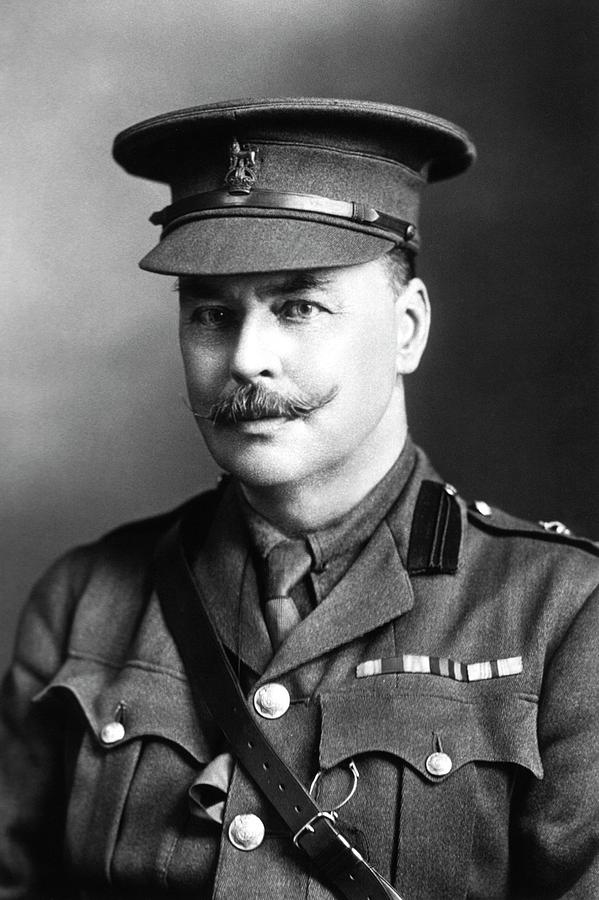
\includegraphics{ronald-ross-national-library-of-medicine.jpg}
% \end{figure}

% \begin{figure}[h]
%   \caption{Dr George Macdonald, 1903-1967}
%   \centering
%   
\includegraphics{george macdonald.jpg}
% \end{figure}

\begin{figure}[H]
  \centering
  \begin{minipage}{.5\textwidth}
    \centering
    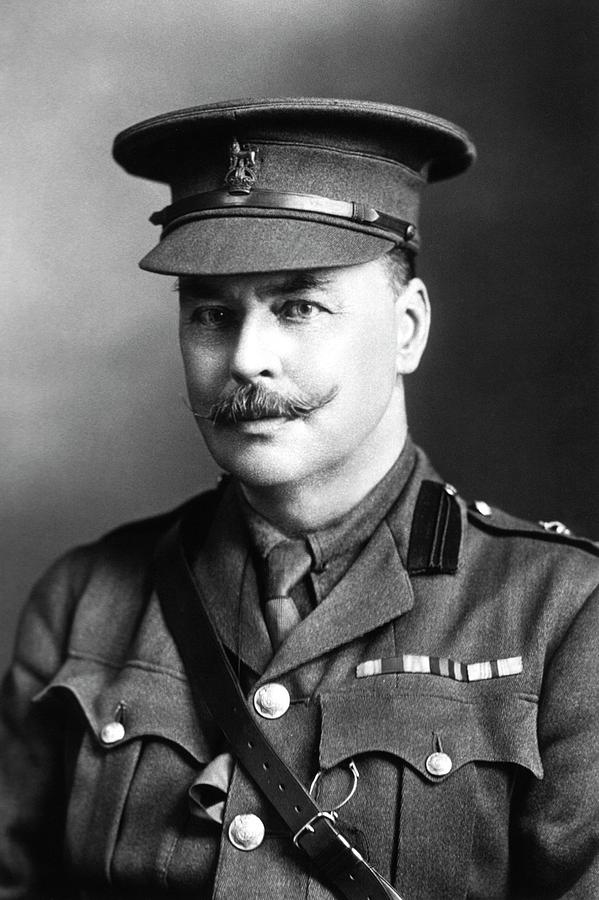
\includegraphics[height=200pt, width=150pt]{ronald-ross-national-library-of-medicine.jpg}
    \caption{Sir Ronald Ross, 1857-1932}
    \label{fig:Ross}
    \end{minipage}%
    \begin{minipage}{.5\textwidth}
    \centering
    
\includegraphics[height=200pt, width=150pt]{george macdonald.jpg}
    \caption{George Macdonald, 1903-1967}
    \label{fig:Macdonald}
  \end{minipage}
\end{figure}

Моделът прави следните допускания (\cite[стр~8,9]{Smith2012}), които се пренасят и в неговите по-сложни варианти, които се разглеждат в дипломната работа:
\begin{enumerate}
  \item Човешката популация и популацията комари е постоянна.
  \item Хората и комарите са разпределени равномерно в средата.
  \item Смъртността от заразата се пренебрегва, както при хората, така и при комарите.
  \item Веднъж заразени, комарите не се възстановяват.
  \item Само податливи се заразяват.
  \item Хората не придобиват никакъв имунитет.
  \item Смъртността на комарите е независима от възрастта им и съответно продължителността им на живот е експоненциално разпределена
  % \item Латентният период при комарите е константен.
\end{enumerate}

\begin{definition}
  \label{def:Parameters}
  Използват се следните означения, които за цел по-лесна четимост се запазват в дипломната работа и за по-сложните модели:
  \begin{itemize}
    \item $X(t)$ е броя заразени с малария хора в момент $t$.
    \item $Y(t)$ е броя заразени с малария комари в момент $t$.
    \item $N$ е човешката популация.
    \item $M$ е популацията от комари.
    \item $\gamma$ е скоростта на оздравяване на хората, т.е. оздравяват след $\frac{1}{\gamma}$ времеви единици.
    \item $\mu$ е скоростта на смъртност на комарите, т.е. умират след $\frac{1}{\mu}$ времеви единици.
    \item $b$ е честотата на ухапване на комарите за единица време.
    \item $\beta_{vh}$ е константна вероятност за заразяване на здрав човек с патогена, когато бъде ухапан от заразен комар, а $\beta_{hv}$ е константна вероятност за заразяване на здрав комар с патогена, когато ухапе заразен човек.
  \end{itemize}
\end{definition}

\begin{remark}
Други типични означения за модели от този вид могат да се намерят в \cite{Smith2012}.
\end{remark}

Моделът се основава на закона за действие на масите.
За интервал $\delta t$, заразените хора ще се получат, като се вземат всички ухапвания на заразени комари за периода и се умножат по вероятността да са по незаразен човек, както и да се предаде патогена, т.е. $\beta_{vh} b Y(t) \frac{N-X(t)}{N} \delta t$, а оздравелите заразени ще са $\gamma X(t) \delta t$, откъдето $\delta X(t) = \beta_{vh} b Y(t) \frac{N-X(t)}{N} \delta t - \gamma X(t) \delta t$.
За този интервал пък заразените комари ще се получат, като се вземат всички ухапвания от незаразени комари и се умножат по вероятнстта да са по заразен човек, както и да се предаде патогена, т.е. $\beta_{hv} b (M - Y(t)) \frac{X(t)}{N} \delta t$, а от тях ще умрат $\mu Y(t) \delta t$, откъдето $\delta Y(t) = \beta_{hv} b (M - Y(t)) \frac{X(t)}{N} \delta t - mu Y(t) \delta t$ След деление на $\delta t$ и граничен преход се достига до следния модел:

\begin{equation}
  \label{eq:BasicProblem}
  \begin{split}
    &\dot{X}(t) = \beta_{vh} b \frac{N-X(t)}{N} Y(t) - \gamma X(t) \\
    &\dot{Y}(t) = \beta_{hv} b \frac{X(t)}{N} (M-Y(t)) - \mu Y(t) \\
  \end{split}
\end{equation}

С помощта на модела Ross показва, че не е необходимо да бъдат изтребени всички комари, за да се изкорени маларията, а само броят им да се сведе под $M^*$:
\begin{equation}
  \label{eq:RossM}
  M^* = \frac{\gamma \mu N}{b^2 \beta_{vh} \beta_{hv}}
\end{equation}

% Прави заключението, че
% \begin{displayquote}
%   As a matter of fact all epidemiology, concerned as it is with the variation of disease from
%   time to time or from place to place, must be considered mathematically, however many
%   variables are implicated, if it is to be considered scientifically at all. To say that a disease
%   depends upon certain factors is not to say much, until we can also form an estimate as to how
%   largely each factor influences the whole result. And the mathematical method of treatment
%   is really nothing but the application of careful reasoning to the problems at issue.
% \end{displayquote}

В модела на Ross фактът, че не всеки заразèн комар е зарàзен, е представен неявно в $\beta_{vh}$.
Допуска се, че инкубационният (латентният) период на комарите $\tau$ е константен.
Така математическото очакване заразèн комар да е станал зарàзен може да се изрази като $e^{-\frac{\tau}{\text{ср. продължителност на живот}}}$.
Но средната продължителност на живот на комарите е точно $\frac{1}{\mu}$, откъдето $e^{-\mu\tau}Y$ е частта зарàзни комари.
Така можеше да разложим $\beta_{vh} = \tilde{\beta}_{vh} e^{-\mu\tau}$, където $\tilde{\beta}_{vh}$ е същинската вероятност за заразяване на човек от комар.
Това е направено в някои от по-нататъшните модели \cite{Smith2012} (като вместо $\tilde{\beta}_{vh}$ се пише $\beta_{vh}$) и затова всички разглеждани модели в дипломната работа ще имат този вид.

\subsection{Модел на Ross-Macdonald с мобилност}
При повече от едно местообитание възниква въпросът как да се броят заразените. В статия на Cosner et al. \cite{Cosner2009} са разгледани два типа модели.
Възможно е да се избере да се разглеждат броя заразени хора и комари във всяко местообитание, като мобилността описва миграция на хора от едно местообитание към друго, като може да се разглеждат популациите в достигнато равновесно състояние.
Другата възможност е да се разглеждат жителите на местообитанията и съответно мобилността да изразява някакви кратки пребивавания на жители от едно местообитание в друго.
По аналогия от хидродинамиката, моделите от първия тип се назовават Ойлерови, а от втория - Лагранжеви.

Разглежда се Лагранжев модел, предложен от Bichara и Castillo-Chavez \cite{Bichara2016}.
Комарите се приема, че не мигрират.
Това се дължи на факта, че повечето комари не се движат повече от няколко десетки до няколко стотици метра за целия си живот \cite{Elbers2015}, като някои от комарите от рода \textit{Anopheles} прелитат и до няколко километра (въведението на \cite{Bichara2016}).
В общия случай от статията са дадени $m$ местообитания с популации на комари и $n$ популации с хора, като всяка от тях е с постоянен размер и хората посещават местообитанията на комарите.
С цел сходство към модела от дипломната работа ще се разгледа случая $n=m=2$, и ще се смята, че местообитанията на комарите съвпадат с това на съответната група хора.

Запазват се означенията от дефиниция \ref{def:Parameters} за модела на Ross \eqref{eq:BasicProblem}, като с долни индекси ще се бележат параметрите на съответното местообитание.
Предполага се, че жителите на местообитание $i$ пребивават в местообитане $j$ за $p_{ij}$ част от времето, $p_{i1} + p_{i2} = 1$.

При направените допускания, в момент $t$, в местообитание $j$ съотношението на заразени към всички хора е:
\begin{equation}
  \frac{p_{1j} X_1(t) + p_{2j} X_1(t)}{p_{1j} N_1 + p_{2j} N_2}
\end{equation}
Ако $b_j$ е броят на ухапвания за човек за единица време, $a_j$ са ухапванията за комар за единица време, то като представим по два начина броя ухапвания в местообитание $j$:
\begin{equation}
  a_j M_j = b_j (p_{1j} N_1 + p_{2j} N_2) \iff b_j = \frac{a_j M_j}{p_{1j} N_1 + p_{2j} N_2}
\end{equation}
Mодел за разпространението на заразата е следния:
\begin{enumerate}
  \item В момент $t$ заразените хора $X_i$ се увеличават от ухапване на незаразен човек от $i$ заразени комари в различните местообитания $j$, а намаляват пропорционално на броя си с коефициента на оздравяване. Заразяването моделираме по закона за масите, като коефициентът за съответните местообитания ще бъде $b_j$. Тогава може да се изрази:
  \begin{equation}
    \dot{X}_i(t) = \sum_{j=1}^{2} \beta_{vh} e^{-\mu_j \tau} b_j p_{ij} (N_i - X_i(t)) \frac{Y_j(t)}{M_j} - \gamma_i X_i(t)
  \end{equation}
  \item В момент $t$ заразените комари $Y_j$ се увеличават от ухапване на заразен човек от някое от различните местообитания $i$ от незаразен комар в местообитание $j$, а намаляват пропорционално на броя си с коефициента на смъртност. Заразяването моделираме по закона за масите, като коефициентът ще бъде $a_j$. Достига се до:
  \begin{equation}
    \dot{Y}_j(t) = \beta_{hv} a_j (M_j - Y_j(t)) \frac{\sum_{i=1}^2 p_{ij} X_i(t)}{\sum_{i=1}^2 p_{ij} N_i} - \mu_j Y_j(t).
  \end{equation}
\end{enumerate}
След като се вземе предвид оценката за $b_j$, то системата има вида:
\begin{equation}
  \label{eq:MigrationProblem}
  \begin{split}
    % &\dot{X}_i(t) = \beta_{vh} (N_i - X_i(t)) \sum_{j=1}^{m} \frac{p_{ij} a_j Y_j(t)}{\sum_{k=1}^n p_{kj} N_k} - \gamma_i X_i(t), \quad i=\overline{1, n} \\
    % &\dot{Y}_j(t) = \beta_{hv} a_j (M_j - Y_j(t)) \frac{\sum_{i=1}^n p_{ij} X_i(t)}{\sum_{i=1}^n p_{ij} N_i} - \mu_j Y_j(t), \quad j=\overline{1, m}
    &\dot{X}_1(t) = \beta_{vh} (N_1-X_1(t)) \left(\frac{p_{11} e^{-\mu_1 \tau} a_1  Y_1(t)}{p_{11} N_1 + p_{21} N_2} + \frac{p_{12} e^{-\mu_2 \tau} a_2  Y_2(t)}{p_{12} N_1 + p_{22} N_2}\right) - \gamma_1 X_1(t) \\
    &\dot{X}_2(t) = \beta_{vh} (N_2-X_2(t)) \left(\frac{p_{21} e^{-\mu_1 \tau} a_1  Y_1(t)}{p_{11} N_1 + p_{21} N_2} + \frac{p_{22} e^{-\mu_2 \tau} a_2  Y_2(t)}{p_{12} N_1 + p_{22} N_2}\right) - \gamma_2 X_2(t) \\
    &\dot{Y}_1(t) = \beta_{hv} a_1 (M_1-Y_1(t)) \frac{p_{11}  X_1(t) + p_{21}  X_2(t)}{p_{11} N_1 + p_{21} N_2} - \mu_1 Y_1(t) \\
    &\dot{Y}_2(t) = \beta_{hv} a_2 (M_2-Y_2(t)) \frac{p_{12}  X_1(t) + p_{22}  X_2(t)}{p_{12} N_1 + p_{22} N_2} - \mu_2 Y_2(t) \\
  \end{split}
\end{equation}

\begin{figure}{}
  \centering
  \begin{tikzpicture}[node distance=20mm]
    % \begin{pgfinterruptboundingbox}
    %   \begin{axis}[ ymin=0, xlabel = variáveis aleatórias, ylabel = frequência]

    \node[label={[xshift=-9mm]\small\it хора}] (sh1) [hostp,text width=22mm] {податливи};

    \node (ih1) [hostp, below of=sh1, text width=22mm] {заразени ($X_1$)};

    \node[label={[xshift=-5mm] \small\it комари}] (sv1) [vectorp, left of=sh1, xshift=-10mm, text width=22mm] {податливи};

    \node (iv1) [vectorp, below of=sv1, text width=22mm] {заразени ($Y_1$)};

    \draw [arrow2] (sh1) -- (ih1);

    \draw [arrow2] (ih1) -- (sh1);

    \draw [arrow] (iv1) -- (sh1) ;

    \draw [arrow] (ih1) -- (sv1) ;

    \draw [arrow2] (sv1) -- (iv1);

    \node[label={[label distance=3mm]-90: местообитание 1},draw=black, fit=(sh1)(iv1),inner sep=5mm, rounded corners](FIt1) {};

    % patch 2

    \node[label={[xshift=-7mm]\small\it хора}] (sh2) [hostp, right of=sh1,xshift=20mm,text width=22mm] {податливи};

    % right
    \node (ih2) [hostp, below of=sh2, text width=22mm] {заразени ($X_2$)};

    \node[label={[xshift=-5mm] \small\it комари}] (sv2) [vectorp, right of=sh2, xshift=10mm, text width=22mm] {податливи};

    \node (iv2) [vectorp, below of=sv2, text width=22mm] {заразени ($Y_2$)};

    \draw [arrow2] (sh2) -- (ih2);

    \draw [arrow2] (ih2) -- (sh2);

    \draw [arrow] (iv2) -- (sh2) ;

    \draw [arrow] (ih2) -- (sv2) ;

    \draw [arrow2] (sv2) -- (iv2);

    \node[label={[label distance=3mm]-90: местообитание 2},draw=black, fit=(sh2)(iv2),inner sep=5mm, rounded corners](FIt2) {};

    % arrows between patches
    \draw [arrow3] (sh1) to (sh2) ;
    \draw [arrow3] (ih1) to (ih2) ;

    % \end{axis}
    % \end{pgfinterruptboundingbox}
    % \path[use as bounding box] ([yshift=-8mm]current axis.south west) rectangle (current axis.north east);
    \end{tikzpicture}
    \centering
    % \captionof{figure}{Диаграма на модела \eqref{eq:MigrationProblem}. \\
    % Черна пунктирана линия: възможен преход на индивид от класа в началото в класа в края.\\
    % Черна непрекъсната линия: индивид от началото може да зарази индивид от края.\\
    % Синя линия: мобилност}
    % Using caption doesn't result in centered text ???
    \caption{Диаграма на модела \eqref{eq:MigrationProblem}.\\
    Черна пунктирана линия: възможен преход на индивид от класа в началото в класа в края.\\
    Черна непрекъсната линия: индивид от началото може да зарази индивид от края.\\
    Синя линия: мобилност}
    \label{fig:TwoPatchModel}
    \end{figure}

% \begin{remark}
%   За съжаление изглежда има анализи в литературата, които \cite{Cosner2009, Agusto2021} не отчитат, че "транзитното" население влияе върху вероятността за ухапване на здрав/заразен човек (т.е. знаменателите в $i$-ия ред на \eqref{eq:MigrationProblem} са просто $N_i$).
%   В случаите когато човешката популация на едното местообитание е много по-голяма от другото (случаят в \cite{Agusto2021}), дори и за малка стойност на мобилността към другото местообитание ще има голямо отклонение между предвижданията на моделите.
% \end{remark}

% \begin{remark}
%   Пример за подробно анализиран Ойлеров модел може се намери в \cite{Prosper2012}.
% \end{remark}

\subsection{Кооперативни(квазимонотонни) системи}
Накратко ще се представят основите свойства на кооперативните системи \cite{Capasso2008}. От тях се нуждаем за някои свойства на модела \eqref{eq:MigrationProblem}.

\begin{definition}[$\leq$-сравнение на вектори]
  Нека са дадени два вектора $\mathbf{v}, \mathbf{w} \in \mathbf{R}^n, \mathbf{v}=(v_1, \cdots, v_n), \mathbf{w}=(w_1, \cdots, w_n)$. Дефинираме релацията $\leq$ в $\mathbf{R}^n \times \mathbf{R}^n$ като:
  \begin{equation*}
    \mathbf{v} \leq \mathbf{w} \iff \forall{i \in \{\overline{1,n}\}}(v_i \leq w_i)
  \end{equation*}
\end{definition}

\begin{definition}[Съкратено означение]
  \label{def:FunctionLEQ}
  Нека $X, Y \subseteq \mathbb{R}^n$. Дефинираме релацията $\leq$ в $\{X \rightarrow Y\}^2$ по следния начин:
  \begin{equation*}
    \mathbf{f} \leq \mathbf{g} \iff \forall_{\mathbf{x} \in X} (\mathbf{f}(\mathbf{x}) \leq \mathbf{g}(\mathbf{x}))
  \end{equation*}
\end{definition}

\begin{definition}(Означение за Якобиан)
  Нека $\mathbf{f}: \mathbb{R}^n \rightarrow \mathbb{R}^m$ е с първи производни по направленията.
  % Якобианът на $\mathbf{f}$ ще се бележи с $\mathrm{D} \mathbf{f} = (\pdv{f_i}{x_j})_{ij}, \mathbf{f} =(f_1, \cdots, f_n)^T$.
  Якобианът на $\mathbf{f}$ ще се бележи с $\mathrm{D} \mathbf{f}$.
\end{definition}

Нека е дадена динамичната система върху интервал от време:
\begin{equation}
  \label{eq:Cooperative}
  \dot{\mathbf{x}} = \mathbf{f}(t, \mathbf{x}),  \quad \mathbf{x} \in \mathbb{R}^n, \mathbf{f} \in C^1(J \times \mathbb{R}^n, \mathbb{R}^n), J \subset \mathbb{R} \text{ е интервал}
  % \mathbb{R}^n \rightarrow \mathbb{R}^n, \quad f \in
\end{equation}

\begin{definition}[Кооперативна система]
  \label{def:Cooperative}
  Системата \eqref{eq:Cooperative} е кооперативна (или още квазимонотонна), ако
  \begin{equation}
    \forall{t \in J}\forall{\mathbf{x} \in \mathbb{R}_{+}^n}\forall{i,j \in \{\overline{1,n}\}}\left(i \neq j \implies \pdv{f_i}{x_j}(t, \mathbf{x}) \geq 0\right)
  \end{equation}
\end{definition}
Кооперативните системи са динамични системи, при които една променлива не може да доведе до понижаване на стойността на друга променлива. Името кооперативна произлиза от моделите за кооперативни междувидови отношения.

\begin{definition}[Квазимонотонна матрица]
  Матрица $A=(a_{ij})_{n \times n}$ е квазимонотонна, ако
  \begin{equation*}
    \forall{i,j \in \{\overline{1,n}\}} \left(i \neq j \implies a_{ij} \geq 0\right)
  \end{equation*}
\end{definition}

\begin{theorem}
  Ако $A$ е квазимонотонна, то винаги има доминантна реална собствена стойност, на която съответства неотрицателен собствен вектор.
\end{theorem}

\begin{definition}[(Не-)разложима матрица]
  Матрицата $A=(a_{ij})_{n \times n}$ e разложима, ако съществува пермутационна матрица $P$, с която:
  \begin{equation*}
    PAP^T =
    \begin{pmatrix}
      B & C \\
      \mathscr{O} & D
    \end{pmatrix}, \quad B, D \text{ - квадратни}
  \end{equation*}
  Матрици, които не са разложими се наричат неразложими.
\end{definition}

\begin{theorem}[Perron-Frobenius]
  Ако $A$ е неразложима, то доминантната ѝ собствена стойност е проста и на нея отговаря положителен собствен вектор $\mathbf{v} \in \mathbb{R}_{+}^n$.
\end{theorem}

\begin{theorem}
  Ако \eqref{eq:Cooperative} е линейна (т.е. $\dot{\mathbf{x}} = A \mathbf{x}, A = (a_{ij})_{n \times n}$) система, то $\mathbb{R}_{+}^n$ е инвариантно.
  Допълнително, ако A е неразложима, то за кое да е $t > 0$ решението е във $\mathrm{int} \mathbb{R}_{+}^n$, стига началното решение да е ненулево, т.е. $\mathbf{x}_0 \neq \mathbf{0}$.
\end{theorem}

Тук виждаме причината кооперативните системи да се наричат квазимонотонни - линейните кооперативни системи са тези с квазимонотонни матрици.

\begin{theorem}[Сравнение на решения]
  \label{thm:Comparison}
  Нека $\mathbf{f}, \mathbf{g} \in C^1(\mathrm{int} \mathbb{R}_{+}^n \mathbb{R}^n)$ са такива, че системите $\dot{\mathbf{x}}=\mathbf{f}(\mathbf{x})$, $\dot{\mathbf{y}}=\mathbf{g}(\mathbf{y})$ са кооперативни, $\mathbf{f} \leq \mathbf{g}$ и $\mathbf{x}_0 \leq \mathbf{y}_0$. Тогава $\forall{t>0}(\mathbf{x}(t) \leq \mathbf{y}(t))$.
\end{theorem}

\begin{definition}[(Не-)разложима система]
  Система \eqref{eq:Cooperative} се нарича (не-)разложима, ако Якобианът на дясната страна $\mathrm{D}\mathbf{f}$ във всяка точка е (не-)разложим.
\end{definition}

\begin{definition}[Силно вдлъбната система]
  Система \eqref{eq:Cooperative} е силно вдлъбната, ако:
  \begin{equation*}
    \mathbf{0} < \mathbf{x}_1 < \mathbf{x}_2 \implies \mathrm{D}\mathbf{f}(\mathbf{x}_2) < \mathrm{D}\mathbf{f}(\mathbf{x}_1)
  \end{equation*}
\end{definition}

\subsection{Свойства на модела на Ross-Macdonald}
Изследвайки системата \eqref{eq:BasicProblem}, Ross веднага забелязва че една равновесна точка е $(0,0)$, а открива, че еднемична е:
\begin{equation}
  E^* = (X^*, Y^*) = \left(N \frac{1 - \frac{\gamma \mu N}{b^2 \beta_{vh} \beta_{hv} M}}{1 + \frac{\gamma N}{b \beta_{vh} M}}, M \frac{1 - \frac{\gamma \mu N}{b^2 \beta_{vh} \beta_{hv} M}}{1 + \frac{\mu}{b \beta_{hv}}}\right)
\end{equation}

Това е и причината да твърди, че заразяване на комари повече от $M^*$ води до ендемия. Наистина, ако $M > M^*$, то числителите в \eqref{eq:RossM} стават отрицателни, откъдето и координатите на $E^*$, а това е физически безсмислено.

Подобно на популационните модели от демографията, може да се дефинира важен параметър $\mathscr{R}_0$, наричан базово число на възпроизводство, който носи смисъла на брой вторични случаи на заразата, причинени от един първичен в популация състояща се единствено от податливи индивиди.
За да може болестта да има ендемично състояние, то е достатъчно $\mathscr{R}_0 > 1$, иначе броят заразени веднага щеше да намалее и съответно нямаше да има равновесна точка, различна от $\mathbf{0}$.

За модела на Ross, репродукционното число може да бъде изведено лесно.
Човек остава заразèн (както и зарàзен) средно $\frac{1}{\gamma}$ време, а пък за единица време средно получава $\beta_{hv} b \frac{M}{N}$ ухапвания от комар, които предават патогена.
Комар остава заразèн за средно $\frac{1}{\mu}$ време и хапе предавайки болестта $\beta_{vh} b$ пъти.
Оттук достигаме до:
\begin{equation}
  \mathscr{R}_0 = \frac{1}{\gamma} \times \beta_{hv} b \frac{M}{N} \times \frac{1}{\mu} \times \beta_{vh} b = \frac{b^2 \beta_{vh} \beta_{hv} M}{\gamma \mu N}
\end{equation}
Но от тази оценка веднага получаваме, че:
\begin{equation}
  \mathscr{R}_0 > 1 \iff M > M^* = \frac{\gamma \mu N}{b^2 \beta_{vh} \beta_{hv}}
\end{equation}
Но това е точно оценката на Ross \eqref{eq:RossM}.

\subsection{Свойства на модела на Ross-Macdonald с мобилност}
За по-сложни модели може да се дефинира базово число на възпроизводство, като ще подходим като van den Driessche и Watmough в \cite{Driessche2002}, основаваща се на идеите в \cite{Diekmann1990}.
Нека имаме групи от заразени $\mathbf{z}$ и $\dot{\mathbf{z}} = \mathbf{G}{\mathbf{z}} = \mathscr{F}(\mathbf{z}) - \mathscr{V}(\mathbf{z})$, където $\mathscr{F}$ определя появата на нови заразени индивиди, а $\mathscr{V}(\mathbf{z}) = \mathscr{V}^-(\mathbf{z}) - \mathscr{V}^+(\mathbf{z})$ е функцията на нетно изменение на популацията, която сме разделили на пристигащи и заминаващи за съответните групи.

\begin{definition}[M-матрица]
  $A = (a_{ij})$ е M-матрица, ако $a_{ij} \leq 0, i \neq j$ и собствените ѝ стойности имат неотрицателни реални части.
\end{definition}

\begin{theorem} \cite[теорема~2]{Driessche2002}
  При изпълнени следните условия:
  \begin{enumerate}
    \item $\mathbf{z} \geq \mathbf{0} \implies \mathscr{V}(\mathbf{z}) \geq 0, \mathscr{V}^+(\mathbf{z}) \geq 0, \mathscr{V}^-(\mathbf{z}) \geq 0$
    \item $z_i = 0 \implies \mathscr{V}_{i}^- = 0$
    \item $\mathscr{F}(\mathbf{0}) = \mathbf{0}, \mathscr{V}(\mathbf{0}) = \mathbf{0}$
    \item Всички собствени стойности на $-\mathrm{D}\mathscr{V}{(\boldsymbol{0})}$ са с отрицателна реална част
    \end{enumerate}
  в сила за репродукционното число е $\mathscr{R}_0 = \rho(F V^{-1})$, където $\rho$ е спектралния радиус, а $F = \mathrm{D} \mathscr{F}(\mathbf{0}), V = \mathrm{D} \mathscr{V}(\mathbf{0})$, където $F \geq \mathscr{O}$, а $V$ е несингулярна M-матрица. \\
  Допълнително, $\mathbf{0}$ е локално асимптотично устойчива, ако $\mathscr{R}_0 < 1$ и неустойчива, ако $\mathscr{R}_0 > 1$.
\end{theorem}

$F_{ij}$ е скоростта, с която индивид от група $j$ заразява индивиди от група $i$, а $(V^{-1})_{jk}$ е средната продължителност на пребиваване на индивид от група $k$ сред индивидите от група $j$, съответно $(F V^-1)_{ik}$ са средния брой новозаразени от $i$ заради индивид от $k$.
% Тук с долни индекси означихме компонентите ма матриците.

В \cite{Bichara2016} с помощта на резултати за кооперативни системи на Smith (виж \cite{Smith1986}) се показва, че за разглежданата от авторите система е изпълнено точно едно от:
\begin{itemize}
  \item $\mathscr{R}_0 \leq 1$. Тогава $\mathbf{0}$ е единствената равновесна точка и е глобално асимптотично устойчива.
  \item $\mathscr{R}_0 > 1$. Тогава $\mathbf{0}$ е неустойчива равновесна точка. Ако системата \eqref{eq:MigrationProblem} е неразложима, има друга равновесна глобално асимптотично устойчива точка.
\end{itemize}

Тъй като $\mathscr{R}_0$ не може да бъде получено в явен вид аналитично, останалата част от статията \cite{Bichara2016} разглежда различни аналитични оценки за $\mathscr{R}_0$ и няколко симулации.

\subsection{Модел на Ross-Macdonald с използване на репелент}
Поради сериозността на заболяването са правени всевъзможни опити за борба с него, като през средата на миналия век от СЗО е създадена Глобалната програма за отстранение на маларията \cite{WHO2017}.
Подход още от древността е изсушаване на блатата, където често се забелязва голямо количество комари.
Както беше споменато самият Ross е предложил изтребване на комарите и основен метод за директно изтребване на комарите са инсектициди, в миналото основно DDT.
За съжаление се забелязва развитие на резистентност към тях.
От друга страна и самите маларийни плазмодии имат резистентност срещу някои от лекарствата \cite[глава~83]{Baron1996}.
Това води до опити за предпазване от комари с репеленти от различен характер, включително такива, които могат да бъдат импрегнирани в тъкани \cite{Grancaric2019}.

Разглежда се модела на Rashkov от \cite{Rashkov2022}.
По същността си уравненията на модела са като на Ross-Macdonald \eqref{eq:BasicProblem}, но с идеята, че може с помощта на репеленти да се намали честотата на ухавания.
Това се моделира с помощта на множител $(1 - \kappa u(t))$ в закона за действие на масите, където $\kappa$ е ефективността на репелента, а пък $u(t)$ функция управление, задаващо пропорцията на хора предпазени с помощта на репелента.

\begin{equation}
  \label{eq:RepellentProblem}
  \begin{split}
    &\dot{X}(t) = \beta_{vh} e^{-\mu \tau} a (1-\kappa u(t)) \frac{N-X(t)}{N} Y(t) - \gamma X(t) \\
    &\dot{Y}(t) = \beta_{hv} a (1-\kappa u(t)) \frac{X(t)}{N} (M-Y(t)) - \mu Y(t) \\
    &u(t) \in \mathscr{U} = \{u:\mathbb{R}_+ \rightarrow [0, \bar{u}] \vert u \text{- измерима}\}
  \end{split}
\end{equation}

Разглежда се следният казус - възможно ли е всички заразени да бъдат хоспитализирани, т.е. да са под $\bar{I}$?
Дефинира се ядрото на слаба инвариантност на Белман:
\begin{equation}
  \label{eq:BasicViability}
  V(\bar{I}, \bar{u}) = \{(X_0, Y_0) \vert \exists{u \in \mathscr{U}}\forall t>0 (X(t) < \bar{I})\}
\end{equation}
С разсъждения сходни на тези, които се правят в следващия раздел на дипломната работа, може да се получи диференциално уравнение, чието решение описва $V(\bar{I}, \bar{u})$ чрез неположителните си линии на ниво \cite{Zidani2013}.
Непосредствено се вижда, че \eqref{eq:RepellentProblem} е кооперативна.
Използвайки теоремата за сравнение на решението може да се докаже разумното предположение, че при възможна по-голяма употреба на репелент или пък по-мощен репелент \eqref{eq:RepellentProblem} ще е с по-голямо ядро на слаба инвариантност.
Симулации, изследващи това са направени в \cite{Rashkov2022}, които показват теоретичните резултати. Може да бъдат видени на следващата фигура.

\begin{figure}[H]
  \centering
  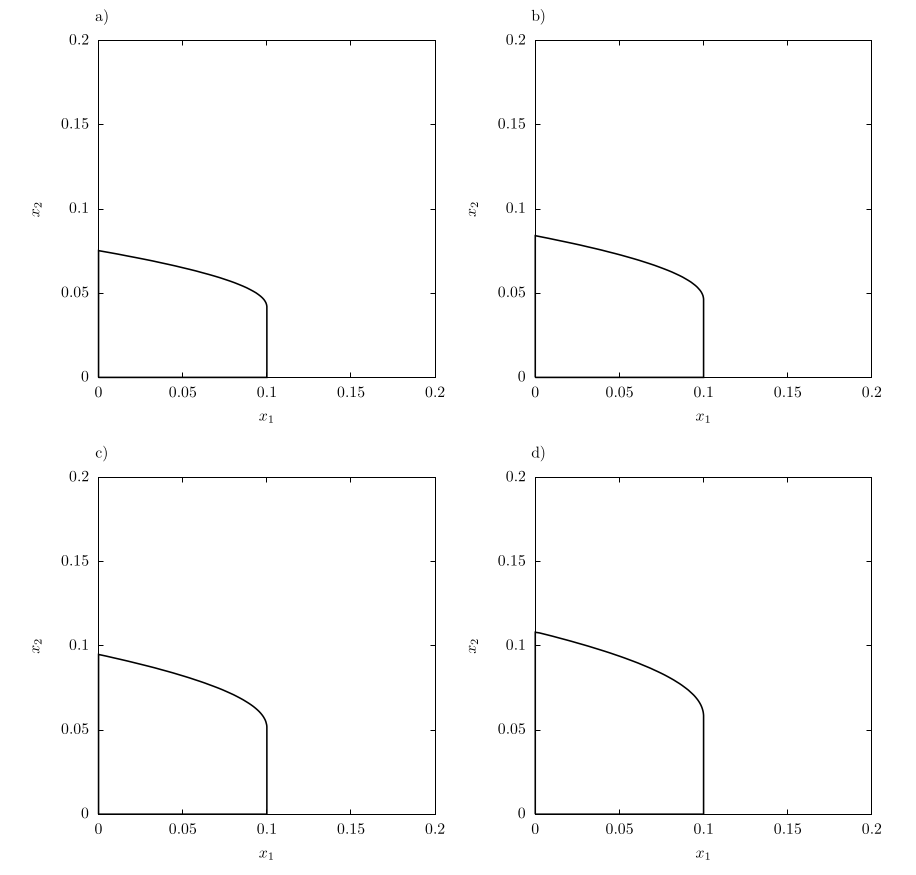
\includegraphics[width=0.7 \textwidth]{rashkov-viability-kernel.png}
  \caption{$V(\bar{I}, \bar{u}), x_1 = \frac{X}{N}, x_2 = \frac{Y}{N}$ за \eqref{eq:RepellentProblem} с $a=0.082, \beta_{hv}=0.1, \beta_{vh}=0.5, \frac{N}{M} = 10, \gamma = \frac{1}{14}, \tau = 10, \mu=\frac{1}{30}, \kappa=0.6, \bar{I}=0.1$ за различни $\bar{u}=0.6 (a),~ \bar{u}=0.7 (b),~ \bar{u}=0.8 (c),~ \bar{u}=0.9 (d)$ (фигурата е взета от \cite{Rashkov2022})}
  \label{fig:RashkovResults}
\end{figure}
